\documentclass{article}
\usepackage[utf8]{inputenc}
\usepackage{amsmath,hyperref,verbatim,listings,graphicx,subfigure,fullpage}

\begin{document}

\title{UML computer project 1}
\author{Juha-Antti Isojärvi \and Mikko Sysikaski}
\maketitle

\section{Exercise 1}
\subsection{}
The plots are shown in Figure~\ref{fig:scatter}. The covariance matrices where generated with the Stetson-Harrison method.
\subsection{}
The principal components of the first and the third point set are shown in Figure~\ref{fig:pcadir}.
\subsection{}
The Figure~\ref{fig:histo} contains the histograms obtained by projecting the points of the first point set on its principal components.
\subsection{}
\subsection{}

\newcommand{\sscale}{0.5}
\begin{figure}
	\centering
	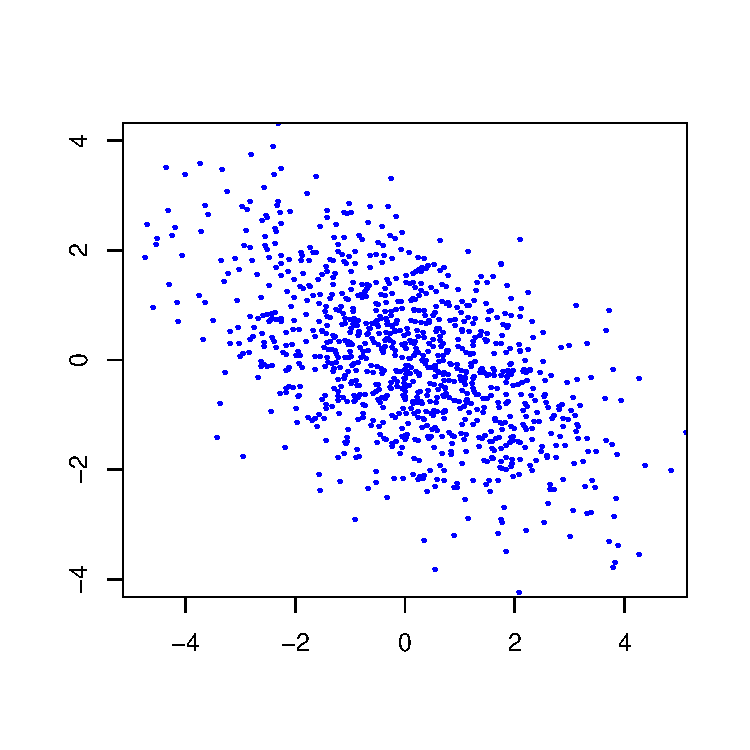
\includegraphics[scale=\sscale]{scatter1}
	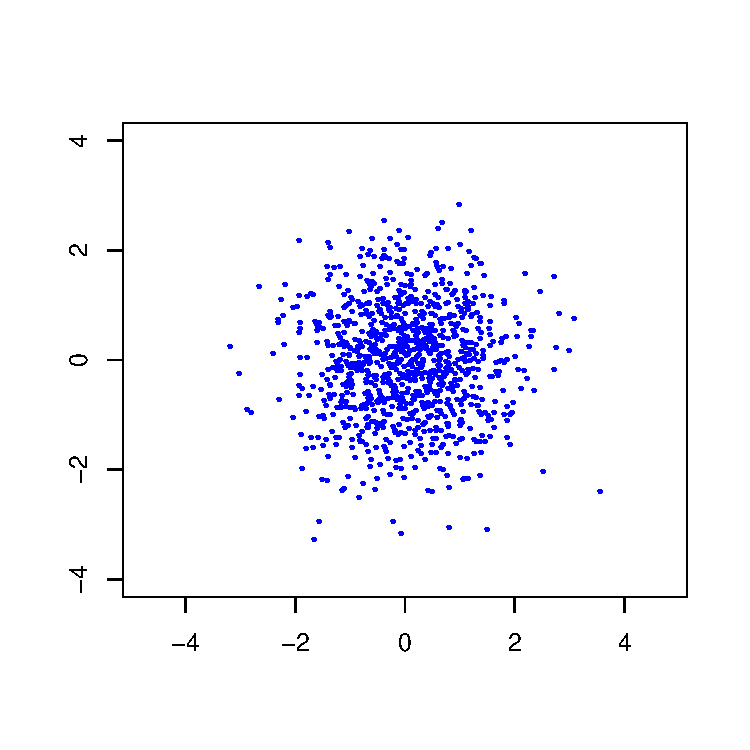
\includegraphics[scale=\sscale]{scatter2}

	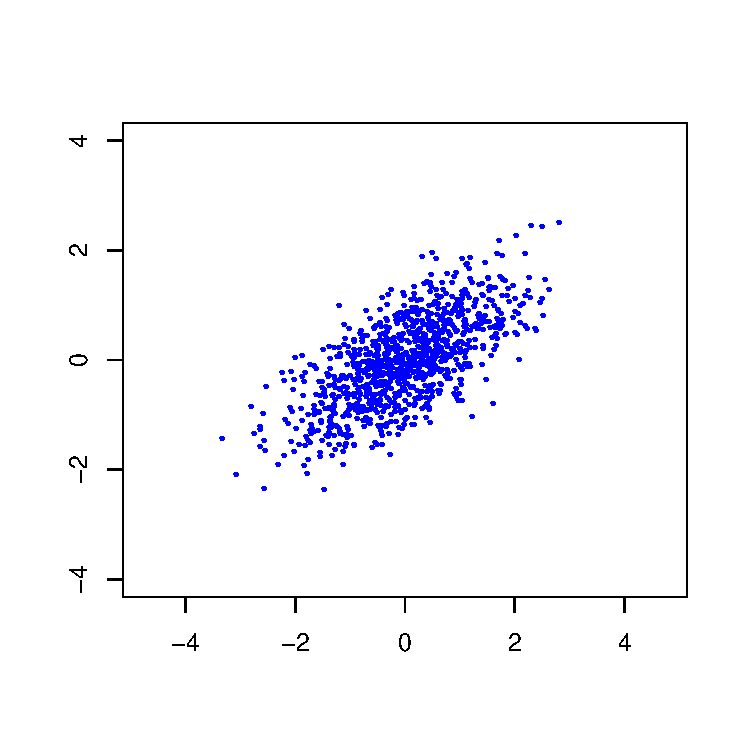
\includegraphics[scale=\sscale]{scatter3}
	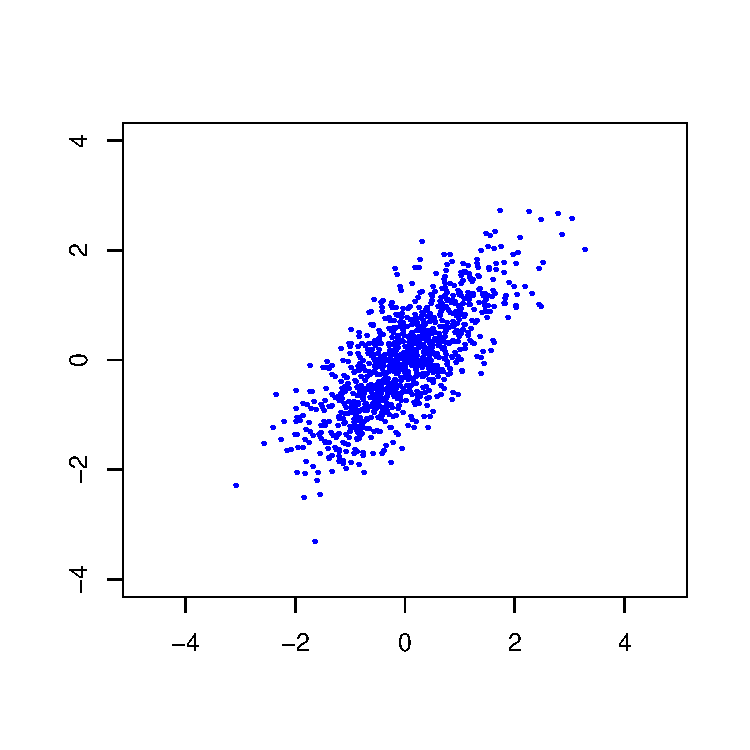
\includegraphics[scale=\sscale]{scatter4}
	\caption{The scatter plots of the data generated in task 1.1.}
	\label{fig:scatter}
\end{figure}
\begin{figure}
	\centering
	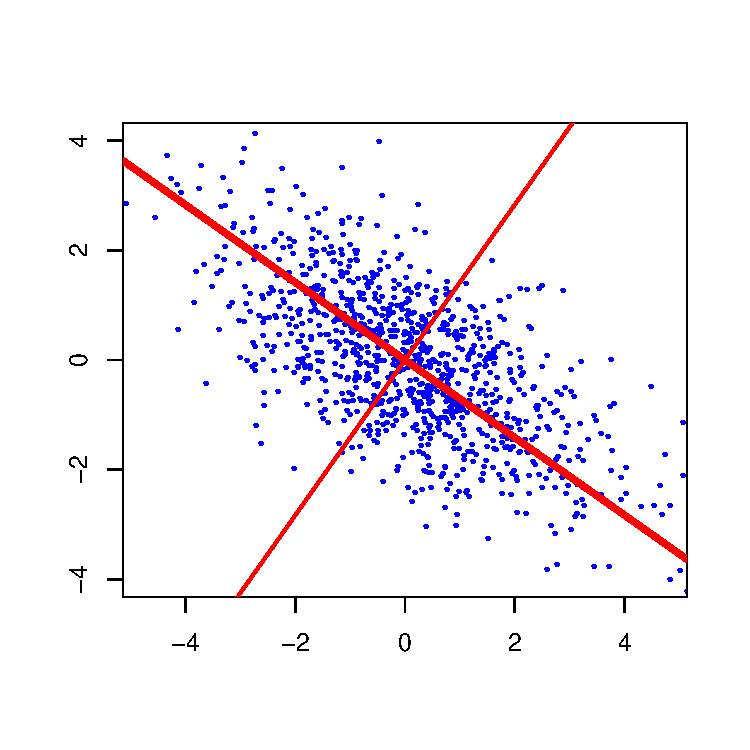
\includegraphics[scale=\sscale]{pcadir1}
	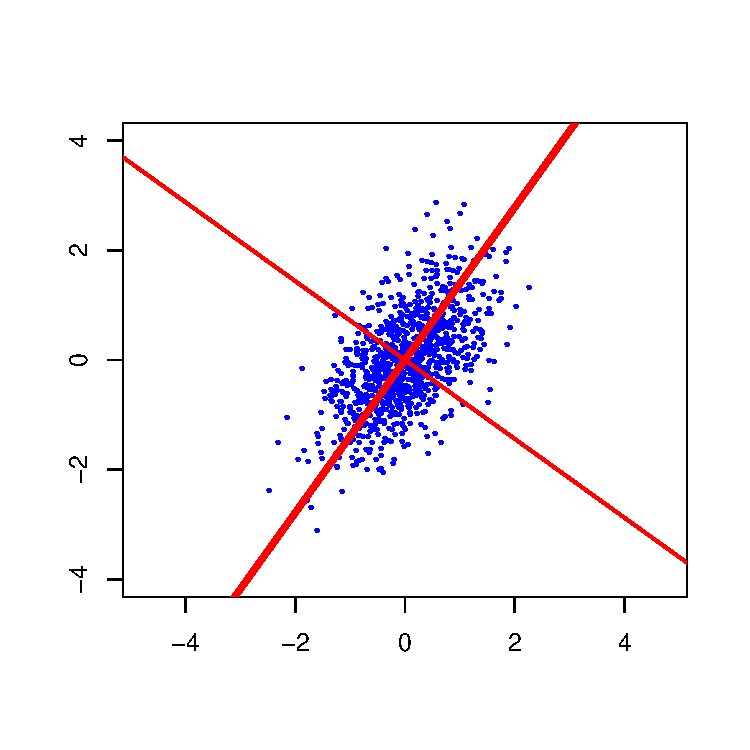
\includegraphics[scale=\sscale]{pcadir3}
	\caption{Principal components of the first and the third point set. The first PC is the bolder line.}
	\label{fig:pcadir}
\end{figure}
\begin{figure}
	\centering
	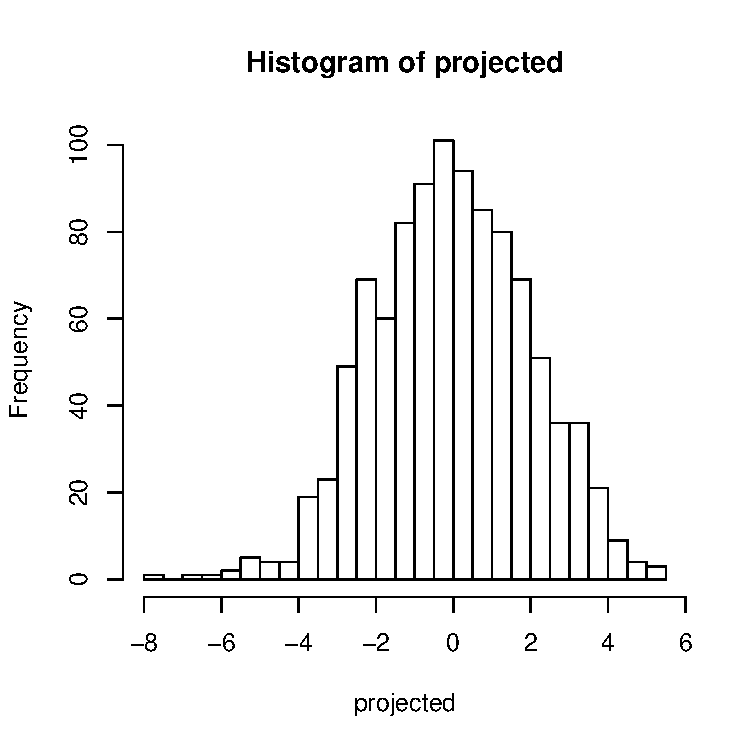
\includegraphics[scale=\sscale]{histo1-1}
	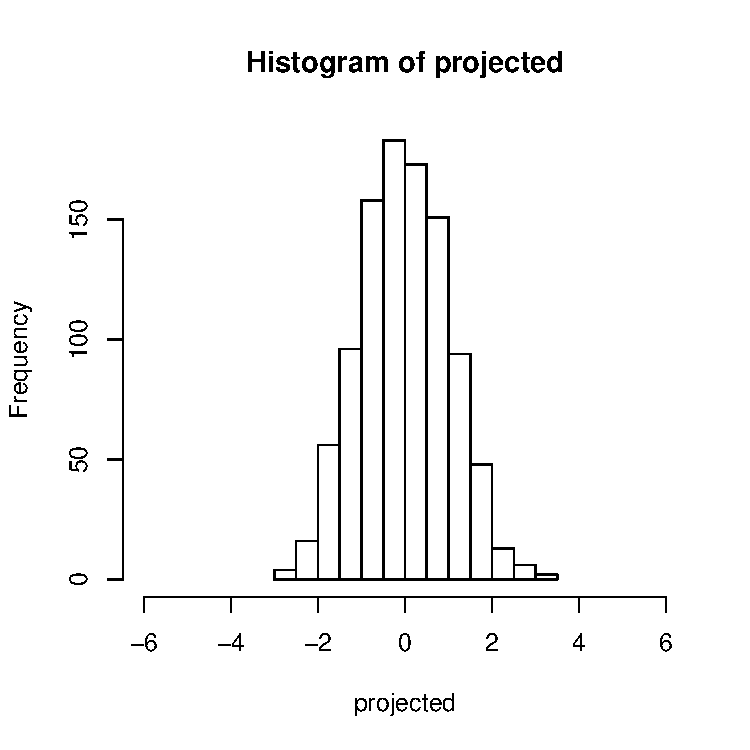
\includegraphics[scale=\sscale]{histo1-2}
	\caption{Histograms of the 1-dimensional data obtained by projecting the points of the first point set on its principal components.}
	\label{fig:histo}
\end{figure}
\begin{figure}
	\centering
	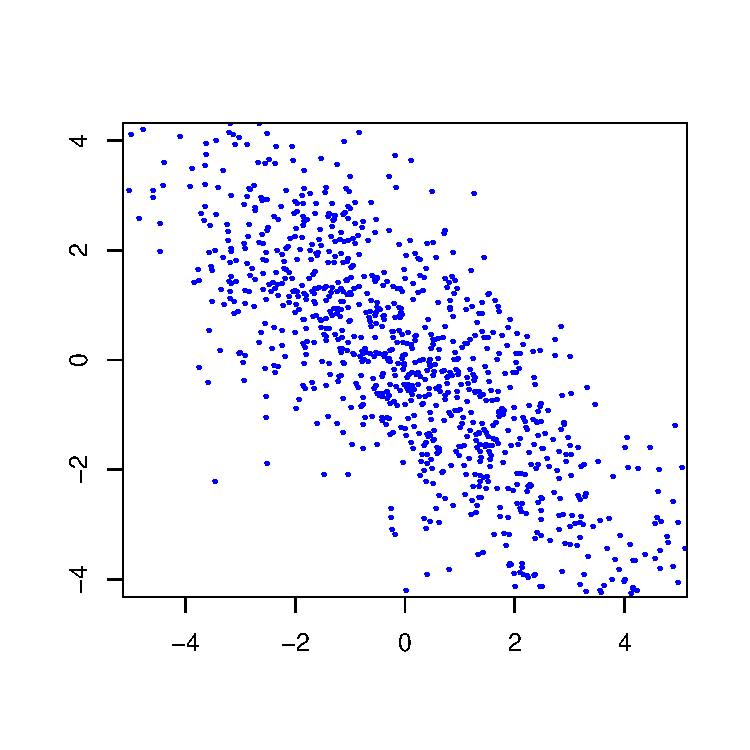
\includegraphics[scale=\sscale]{vscatter}
	\caption{}
	\label{fig:vscatter}
\end{figure}
\begin{figure}
	\centering
	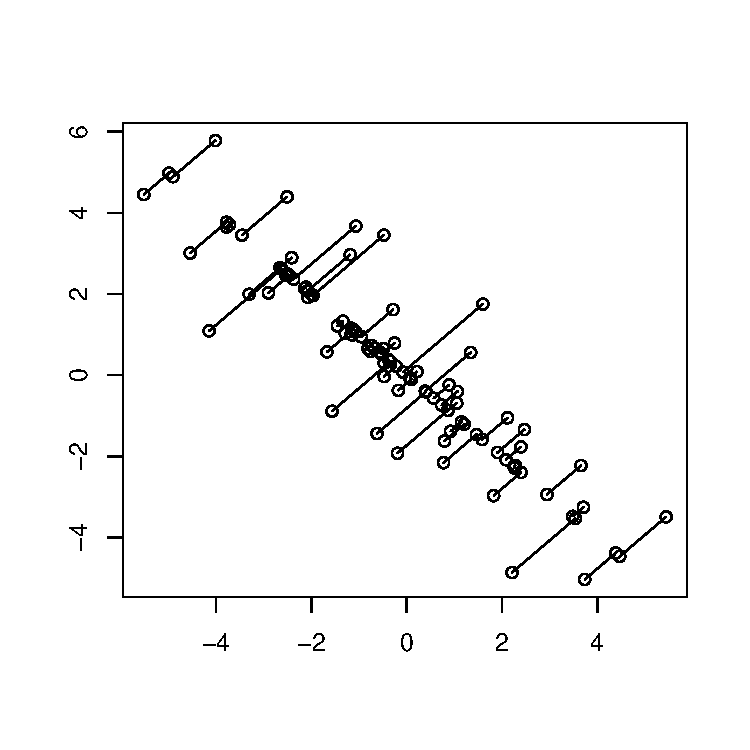
\includegraphics[scale=\sscale]{proj}
	\caption{}
	\label{fig:proj}
\end{figure}

\end{document}
